% !TEX encoding = UTF-8 Unicode

\documentclass[a4paper]{article}

\usepackage{color}
\usepackage{url}
\usepackage[T2A]{fontenc} % enable Cyrillic fonts
\usepackage[utf8]{inputenc} % make weird characters work
\usepackage{graphicx}

\usepackage[english,serbian]{babel}
%\usepackage[english,serbianc]{babel} %ukljuciti babel sa ovim opcijama, umesto gornjim, ukoliko se koristi cirilica

\usepackage[unicode]{hyperref}
\hypersetup{colorlinks,citecolor=green,filecolor=green,linkcolor=blue,urlcolor=blue}

%\newtheorem{primer}{Пример}[section] %ćirilični primer
\newtheorem{primer}{Primer}[section]

\begin{document}

\title{3D stampa\\ \small{Seminarski rad u okviru kursa\\Tehničko i naučno pisanje\\ Matematički fakultet}}


\author{    Nevena Miletic\\ mi22193@alas.matf.bf.ac.rs
        \and Matija Todorovic\\ mi22282@alas.matf.bf.ac.rs
        \and Djordje Sajic\\ mi22237@alas.matf.bf.ac.rs
        \and Relja Gajic\\ mi22131@alas.matf.bf.ac.rs
 }

\date{10.novembar 2022.}
\maketitle
\abstract{
Aditivna proizvodnja je moderna tehnologija proizvodnje trodimenzionalnih objekata. 3D štampa predstavlja generalno brže, jeftinije i lakše rešenje od drugih tehnologija proizvodnje 3D objekata. Omogućava izradu maketa delova i sklopova od više različitih materijala, različitih mehaničkih i fizičkih svojstava u jedinstvenom procesu. Ova tehnologija proizvodi modele koji verno oponašaju izgled, utisak i funkcionalnost proizvoda prototipa. U poslednjih nekoliko godina 3D štampači su postali finansijski dostupni malim i srednjim preduzećima, čime se izrada prototipa pomera iz teške industrije i u kancelarijsko okruženje.Iako su pomenute
mašine do skora bile dostupne samo malom broju ljudi, uglavnom naučnicima, to više nije slučaj. Cena 3D štampača su sve niže. Vremenom mogućnosti koje ovi uredjaji pružaju polako postaju neograničene.
\tableofcontents

\newpage

\section{Uvod}
\label{sec:uvod}
Aditivna proizvodnja predstavlja način proizvodnje gde se iz digitalnog modela stvara trodimenzionalan predmet. Kako to zapravo izgleda?
\bigbreak

3D štampa može da se zamisli kao štampa tankih horizontalnih slojeva. Ti slojevi predstavljaju horizontalni presek predmeta.
\bigbreak Tehnologija je nastala 80-ih godina prošlog veka i koristila se pre svega za proizvodnju prototipova. Ipak, od tada 3D štampa počinje da se koristi kao tehnika za stvaranje proizvoda gotovo u svim industrijama.
Proizvodi koji se 3d štampaju mogu biti od različitih materijala, od plastike, preko keramike, do metala. Tehnologija se i dalje razvija a novi materijali pomoću kojih se štampa se uvode neverovatnom brzinom. Sada je moguće i istovremeno uklapanje različitih vrsta materijala. Osim izrade prototipova, 3D štampači nude veliki potencijal za proizvodnju različitih aplikacija u oblasti proizvodnje nakita, obuće, industrijskog dizajna, arhitekture, automobilske industrije, avio, stomatološke i medicinske industrije.

\section{Istorija razvoja 3D stampe}


\bigbreak Možda ste čuli za 3D štampu koja je proglašena budućnošću proizvodnje. I sa načinom na koji se tehnologija razvija i širi komercijalno, može se vrlo dobro nadoknaditi u oprezu koja ga okružuje. Šta je 3D štampanje? A ko je to izmislio? 
\bigbreak Najbolji primer na koji mogu da se setim kako opisuje kako 3D štamparski radovi dolaze iz TV serije Star Trek: The Next Generation. U tom fiktivnom futurističkom univerzumu, posada na brodu svemirskog broda koristi mali uređaj koji se zove replikator za stvaranje skoro bilo čega, kao u bilo čemu od hrane i pića do igračaka. 
\bigbreak Sada, dok oba mogu da izvedu trodimenzionalne objekte, 3D štampanje nije skoro toliko sofisticirano. Pošto replikator manipuliše subatomske čestice kako bi proizveo bilo koji mali objekat, 3D štampači "štampaju" materijale u sukcesivnim slojevima kako bi formirali objekat. 
\bigbreak Istorijski gledano, razvoj tehnologije počinje početkom 1980-ih godina, čak i predavanje TV emisije. 1981. godine, Hideo Kodama iz Instituta za industrijska istraživanja Nagoya prvi je objavio račun o tome kako se materijali koji se nazivaju fotopolimeri koji su ojačani prilikom izlaganja UV zračenju mogli iskoristiti za brzo izradu čvrstih prototipova. Iako je njegov članak postavio temelje za 3D štampanje, on nije prvi napravio 3D štampač. 
\bigbreak Ta prestižna čast ide na inženjer Chuck Hull-a, koji je dizajnirao i napravio prvi 3D štampač 1984. radio je za kompaniju koja je koristila UV lampe za oblikovanje čvrstih, izdržljivih premaza za stolove kada je pogodio ideju da iskoristi ultraljubičastu tehnologija za izradu malih prototipova. 
\bigbreak Ključ za izradu takvog štampača bili su fotopolimeri koji su ostali u tečnom stanju sve dok nisu reagovali na ultraljubičastu svetlost. Sistem koji je Hull na kraju razvio, poznat kao stereolitografija, koristio je UV zračenje kako bi skicirao oblik objekta iz kadra tečnih fotopolimera. 
\bigbreak On je patentirao tehnologiju 1984. godine, ali je tri nedelje nakon što je tim francuskih pronalazača Alain Le Méhauté, Olivier de Witte i Jean Claude André podnio patent za sličan proces. Međutim, njihovi poslodavci napustili su napore da dalje razviju tehnologiju zbog "nedostatka poslovne perspektive". To je omogućilo Hullu da autorsko pravo pod pojmom "Stereolithography". Njegov patent, naslovljen "Aparat za proizvodnju trodimenzionalnih objekata stereolitografijom" objavljen je u martu 11, 1986. Te godine, Hull je takođe formirao 3D sisteme u Valensiji, Kalifornija, tako da on može započeti brzo prototipiranje komercijalno. 
Dok je Hullov patent obuhvaćao mnoge aspekte 3D štampanja, uključujući dizajn i operativni softver, tehnike i razne materijale, drugi izumitelji bi se nadovezali na koncept sa različitim pristupima. 1989. godine dodeljen je patent Carlu Deckardu, diplomantu Univerziteta u Teksasu koji je razvio metod pod nazivom selektivno lasersko sinterovanje. Sa SLS-om, laserski zrak se koristi za prilagođavanje praškastih materijala, kao što je metal, zajedno kako bi se formirao sloj objekta. 
\bigbreak Svježi prah bi se dodao na površinu nakon svakog uzastopnog sloja. Ostale varijacije kao što su direktno metalno lasersko sinterovanje i selektivno lasersko taljenje se takođe koriste za izradu metalnih predmeta. 
\bigbreak Najpopularniji i najprepoznatljiviji oblik 3D štampanja naziva se modeliranje spojenih depozita. FDP, koji je razvio pronalazač S. Scott Crump, postavlja materijal u slojeve direktno na platformu. Materijal, obično smola, se isprazni kroz metalnu žicu i, nakon puštanja kroz mlaznicu, odmah se ojača. Ideja je došla u Crump 1988. godine, dok je pokušavao da napravi igračku žabu za svoju žerku izdavanjem voska za sveće pomoću pištolja za lepak. 
\bigbreak 1989. godine Crump je patentirao tehnologiju i sa svojom suprugom soustanovio Stratasys Ltd. za proizvodnju i prodaju 3D štamparskih mašina za brzo prototipiranje ili komercijalnu proizvodnju. 
Kompaniju su uzeo u javnost 1994. godine, a do 2003. godine FDP je postao najprodavanija tehnologija brze prototipizacije. 

\section{Tehnike 3D stampe}
\label{sec:naslov1}
Prema tehnici 3D štampanja možemo razlikovati sledece tehnologije:
\begin{itemize}
\item \textbf{Inkjet}
\item \textbf{Fused Deposition Modelin(FDM)}
\item \textbf{Stereolitografija}
\item \textbf{Selektivno lasersko sinterovanje (SLS)}
\item \textbf{Proizvodnja objekata laminacijom (LOM)}
\end{itemize} 



 


\subsection{Inkjet}
\label{subsec:podnaslov1}
Inject - креира проторип на основу 3D модела тако што прави слој по слој пројекта.
\bigbreak Истиче се по атрибуту да је адаптиван на разне облике течних материјала што пружа стварање кондуктивних или изолационих структура у високој резолуцији. 
\bigbreak За разлику од процеса који користе фузију металних или пластичних материјала, инјект штампању није потребно додатно прерађивање и обрада нако извршеног штампања.
\begin{center}
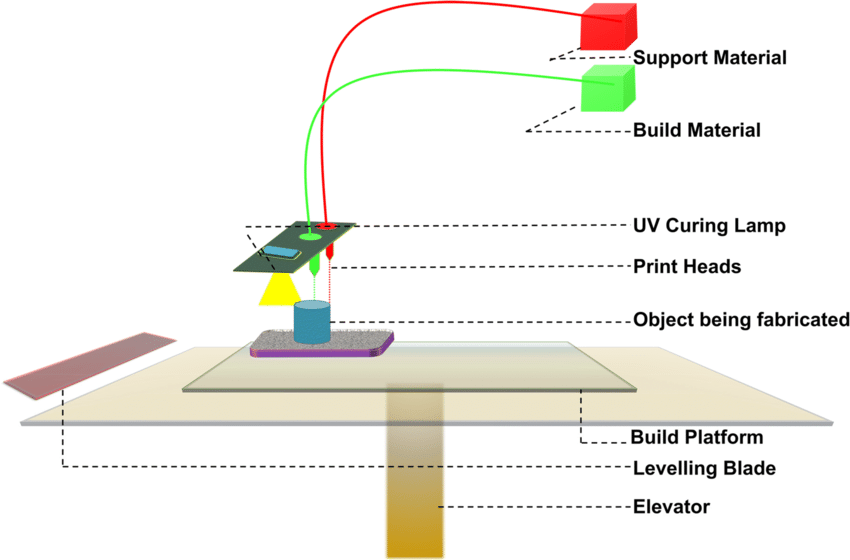
\includegraphics[width=.5\textwidth ]{Tehnikeslike/Inject.png}
\end{center}

\subsection{Fused Deposition Modelin(FDM)}
\label{subsec:podnaslov2}
FDM (Fused Deposition Modeling) - представља најкоришћену и најјефтинију технику за 3D штампање. Лак је за коришћење, он користи термопластичне филаменте са ектрузијом између сваког слоја.
\bigbreak Најчешће се користи у девелоповању производа  и тест модела који инжињери користе да провере да ли облиk одговара датом уређају по димензијама. 
\bigbreak Састоји се од подлоге на којој се извршава штампање, дисплеја за штампање, машине која загрева филаменте и кулера који одржава температуру уређаја.

\begin{center}
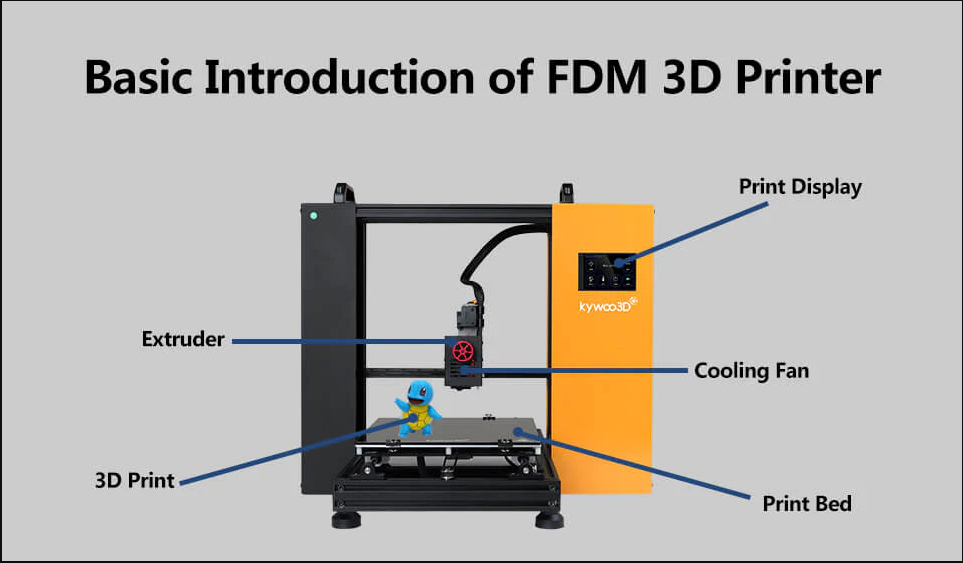
\includegraphics[width=.5\textwidth ]{Tehnikeslike/FDM.PNG}
\end{center}

\subsection{Stereolitografija}
\label{subsec:podnaslov3}
Stereolitografija (Stereolithography) -познатија као SLA, користи резервоар течног фотополимера који формира слој по слој пројекта , где се након формирања сваког слоја полимер стврдне уз помоћ ултраљубичастог светла.
\bigbreak Након сваког одрађеног слоја подлога се спушта како би кренула обраду следећег.Када се заврши обрада 3D модела потребно је извршени пројекат опрати растварачем да би се уклонила течнос опасна по живот.
\bigbreak Ова техника се најчешће користи за креирање 3D модела високих резолуција.  Стереолитографија користи помоћне стубове који спречавају да дође до деформације приликом изградње следећих слојева који се налазе изнад њега.

\begin{center}
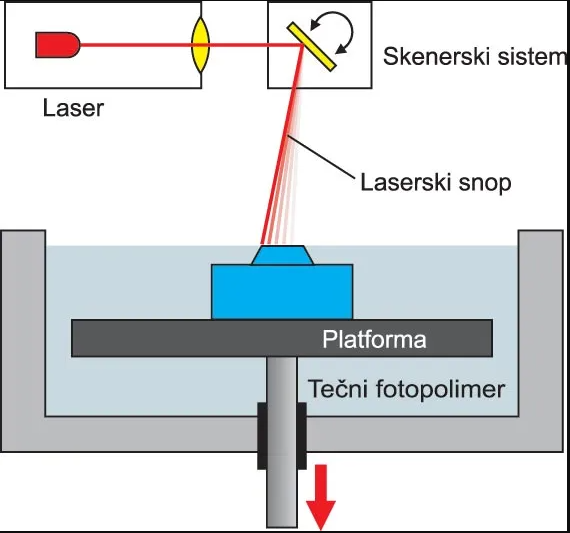
\includegraphics[width=.5\textwidth ]{Tehnikeslike/Stereolitografija.PNG}
\end{center}

\subsection{Selektivno lasersko sinterovanje (SLS)}
\label{subsec:podnaslov4}
Selective Laser Sintering (SLS) - користи се за прављење прототипа од метала и пластике. Уз помоћ powder beds машина прави дизајнове слој по слој, при чему користи  ласер грејање и збијање (синтеровање) праха датог материјала. 
\bigbreak Након сваког слоја постоље се спушра и додаје нови слој материјала све док машина не заврши изградњу модела. Пошто чврстина модела зависи од највеће температуре машине SLS загреје превремено прах на powder bed-у испод њене температуре топљења да направи лакше ласеру да повећа температуру одређене регије. 
\bigbreak Овај процес захтева помоћне стубове који служе да не дође до дефекта виших слојеба модела приликом изграде.

\begin{center}
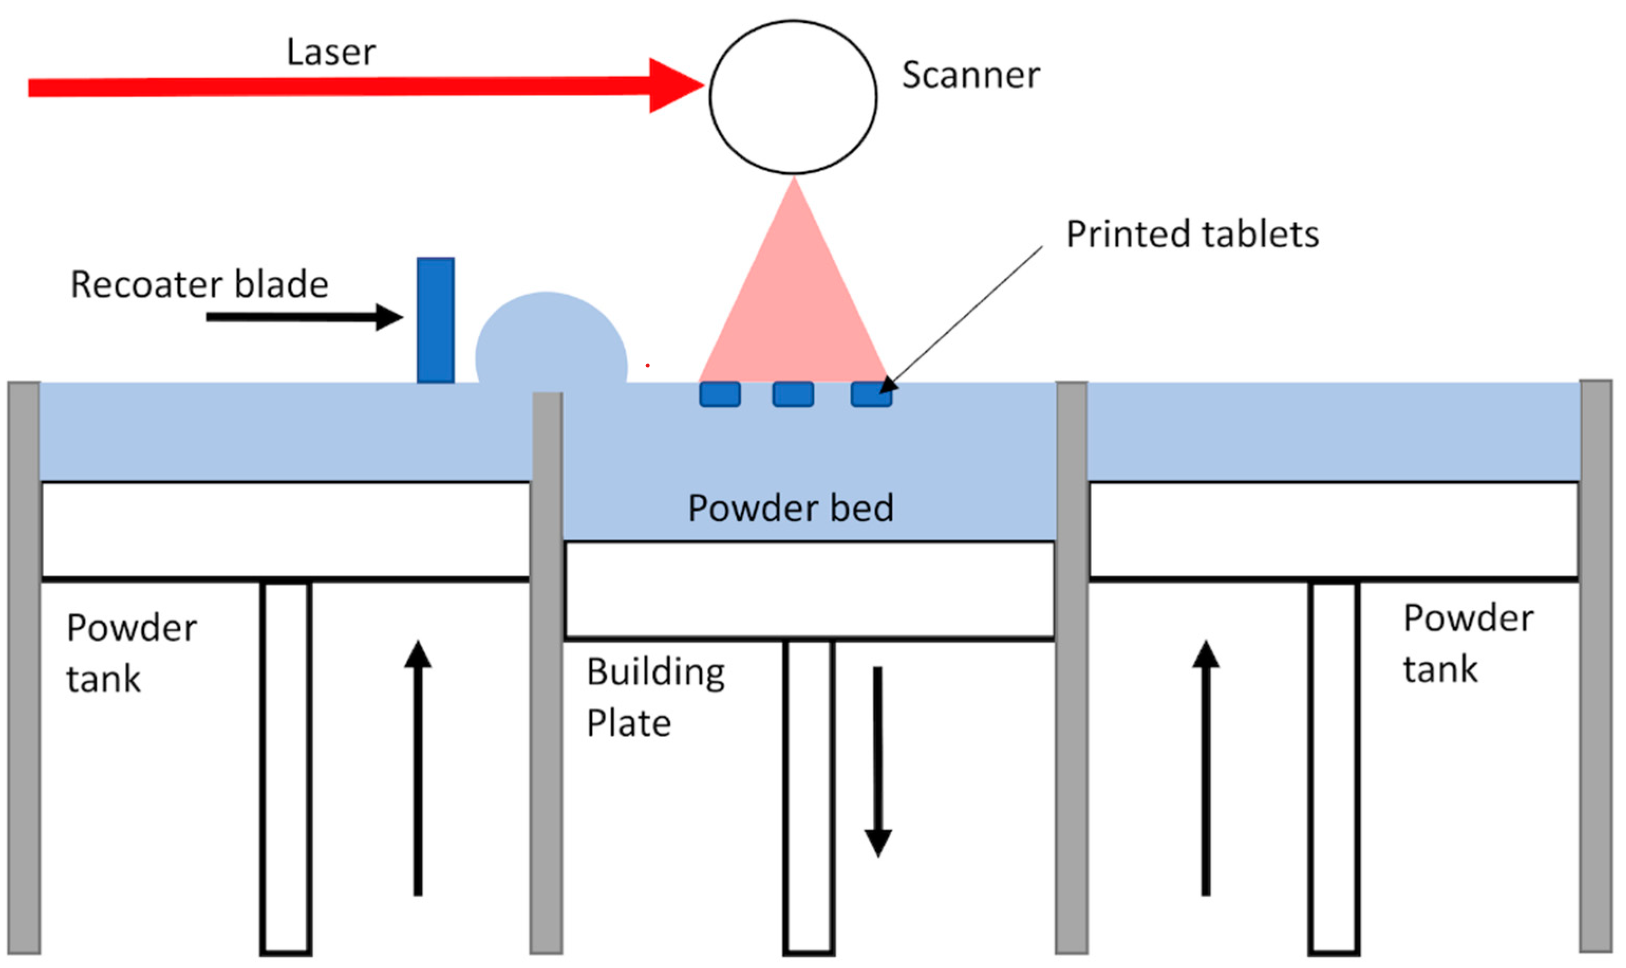
\includegraphics[width=.5\textwidth ]{Tehnikeslike/Sls.png}
\end{center}

\subsection{Proizvodnja objekata laminacijom (LOM)}
\label{subsec:podnaslov5}
Proizvodnja objekata laminacijom (Laminated object manufacturing) - скраћено LOM, користи папир премазан лепком, пластику или метални ламинат као медијум за 3D штампање. 
\bigbreak Хартије од датог материјала су залепљене једна за другу слој по слој и исечене у облик користећи нож или ласер. Након тог процеса оне се могу додатно дорадити шмирглањем и бушењем ако је потребно.

\begin{center}
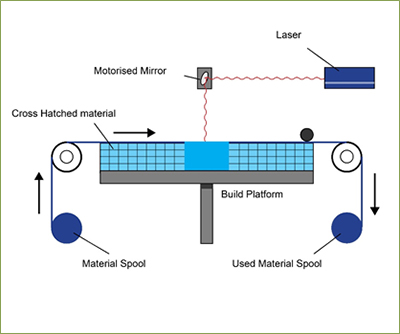
\includegraphics[width=.5\textwidth ]{Tehnikeslike/LOM.jpg}
\end{center}

\newpage

\section{Primena}
\label{sec:Primena}

U proteklih nekoliko godina, štampači postaju sve dostupniji i dostupniji. Više se ne koriste isključivo u teškoj industriji, već i u manjim preduzećima i čak i za ličnu upotrebu. Koriste se u najrazličitije svrhe i skoro svim granama privrede. Kao što je već napomenuto, broj raznovrsnih materijala koji se koriste za rad sa 3d štampačima je ogroman i raste vrtoglavom brzinom. To omogućava veliku raznovrsnost njihove primene. 

\subsection{Medicina}
\label{subsec:podnaslov6}

Primena 3d štampača u medicini je počela 2014. godine u Velikoj Britaniji kada je pacijentu koji je od posledica raka izgubio gotovo pola kože lica, upravo putem 3d štampe napravljen novi deo lica i postavljen na mesto starog. Ovo predstavlja veliki korak u modernoj medicini jer se prvi put dogodilo da je čovek u mogućnosti da odštampa neki deo svog tela. 
\bigbreak Ovakvi procesi se izvršavaju primenom fotogrametrije. Proces se sastoji iz niza kamera koje prave fotografije zdravih tkiva pacijenta, a zatim ga računarski sklapaju u jednu 3d celinu koja će kasnije biti odštampana. Proces slikanja i izrade celine je vrlo brz i traje svega nekoliko sati, dok je proces štampanja vrlo delikatan i sa veoma malim prostorom za grešku, naravno, traje znatno duže od prethodnih. Pričvršćivanje novog, štampanog tkiva se izvršava hirurškim zahvatom.

\subsection{Prototipovi}
\label{subsec:podnaslov7}

Ovo je najvažniji i najrasprostranjeniji vid primene 3d štampača. Dizajnerima je znatno olakšan i ubrzan rad. Štampač može uz korišćenje male količine materijala i u kratkom vremenskom roku da stvori prototip za čiju bi izradu bilo potrebno značajno više. Ovaj vid primene se koristi u gotovo svim granama privrede.

\subsection{Vojna primena}
\label{subsec:podnaslov8}

Naravno, ljudi su vrlo brzo našli primenu 3d štampačima u vojnoj industriji. Konkretno, za izradu delova za pištolje i puške, kao i za izradu bojeve municije. Počelo je tako što je jedan mladi amerikanac došao na ideju da napravi jeftine delove za svoju pušku, što mu je i pošlo za rukom. Ono što je izuzetno privlačno kompanijama za proizvodnju oružja, kao i vladama i organizacijama koje ga kupuju, je upravo mogućnost pravljenja oružja kome se ne može ući u trag. U vojnoj industriji se očekuje najveći porast primene štampača. 

\subsection{Izrada odeće i obuće}
\label{subsec:podnaslov9}

Razne kompanije za proizvodnju odeće i obuće obilato koriste 3d štampače. Ne toliko za pravljenje konkretnih celina kao što su patike, već za pravljenje raznih manjih delova. Poznati su upravo delovi za sportsku odeću poput krampona za kopačke ili ojačanih vrhova pertli. 

\end{document}
